\begin{frame}{A background symbol also earns reconstruction credit}
\key{Our challenge}\par
A triangle beside a 7 contributes to the pixel loss. Its shape adds no intended information about digit identity.
\par\bigskip
\key{Our research question}\par
We measure the accuracy DEC and IDEC lose when geometric symbols appear, and test whether a spatial prior reduces that loss for IDEC.
\notefoot{The cluster of interest is digit identity. Digit labels enter evaluation after training.}
\end{frame}

\begin{frame}{The generator varies the background of the same digit}
\centering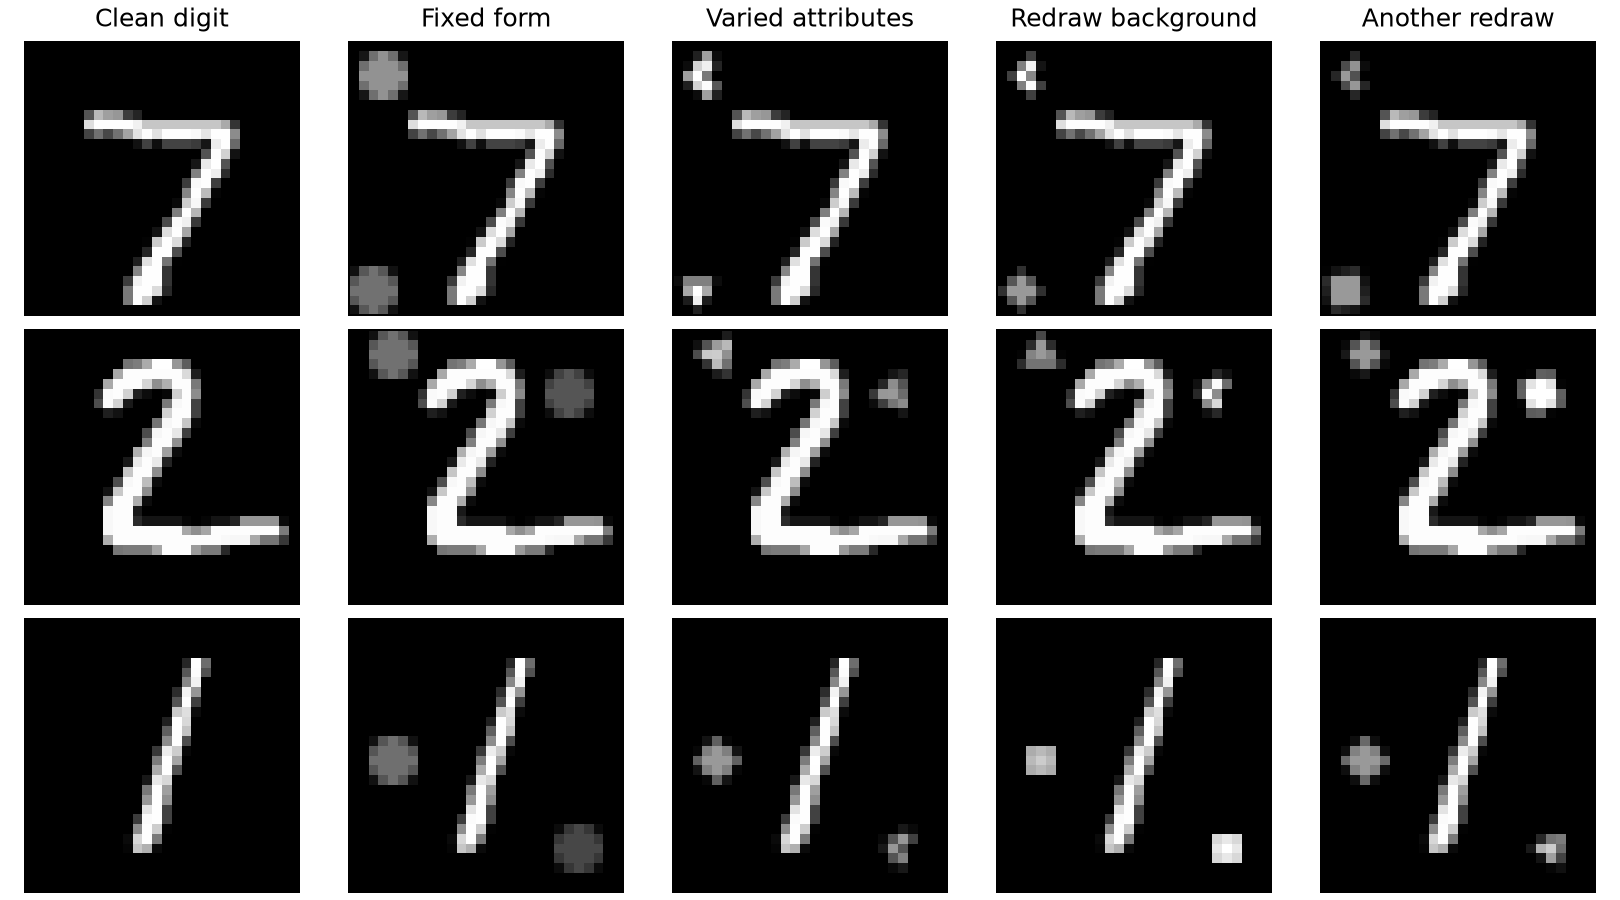
\includegraphics[height=.72\textheight,width=.95\linewidth,keepaspectratio]{../figures/varied.png}
\notefoot{Two symbols, 96 combinations of shape, size, rotation and brightness. The bounding boxes leave a one-pixel margin around every digit stroke. Test redraws retain the original symbol positions.}
\end{frame}

\begin{frame}{What happens when the decoder can omit the symbols?}
\key{Same marked inputs, different reconstruction targets}\par
Two models see the same digits with the same symbols. One reconstructs the full image. The other reconstructs the clean digit provided by the generator.
\par\bigskip
\centering\small\begin{tabular}{llrrr}
\toprule
Pretrain target & Fine-tune target & Marked ACC & Redraw flips & Decoder response\\
\midrule
Full & Full & 65.40 & 2.98 & 0.00828\\
Full & Clean & 66.85 & 2.65 & 0.00159\\
Clean & Full & 70.62 & 2.51 & 0.00289\\
Clean & Clean & 71.44 & 2.35 & 0.00145\\
\bottomrule
\end{tabular}

\notefoot{Earlier target ablation, five seeds. Clean targets in both stages raised marked ACC by 6.04 points. The clean image is extra training information available for this diagnostic.}
\end{frame}

\begin{frame}{Our solution weights reconstruction by likely relevance}
MNIST handwriting tends to lie near the center. A Gaussian weight gives errors on central pixels more influence on the loss.
\par\medskip
\centering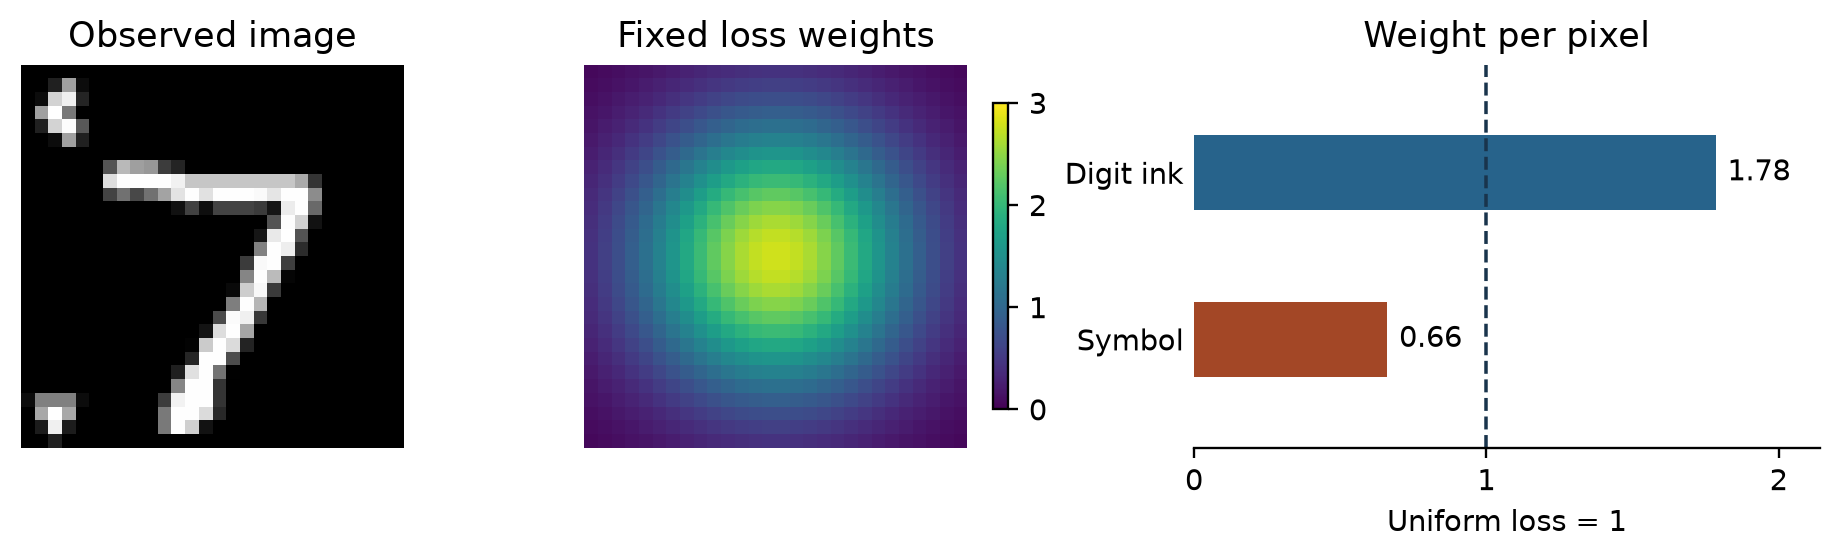
\includegraphics[width=.92\linewidth,height=.44\textheight,keepaspectratio]{../figures/gaussian_prior.png}
\notefoot{We apply the same fixed map to every image. The target is the observed image. The mean pixel weight is one and the width is seven pixels. The ink/symbol split is used only to audit the prior.}
\end{frame}

\begin{frame}{DEC and IDEC start from identical weights and centers}
\begin{columns}[T,onlytextwidth]
\column{.48\textwidth}\key{Inside each training domain}\par\medskip
Pretrain one autoencoder and fit K-means. Fork DEC with only clustering KL and IDEC with the same KL plus pixel MSE. Train for the same 5,600 updates.
\column{.47\textwidth}\key{Across domains}\par\medskip
Repeat on clean and marked versions of the same digits. For each method and seed, subtract marked accuracy from clean accuracy. Compare those losses within seed.
\end{columns}
\par\bigskip
\notefoot{12,000 training and 10,000 held-out digits per domain. Standard DEC uses autoencoder pretraining. An additional control skips that stage and uses only KL from a random start.}
\end{frame}

\begin{frame}{Which model loses more accuracy to the background?}
\centering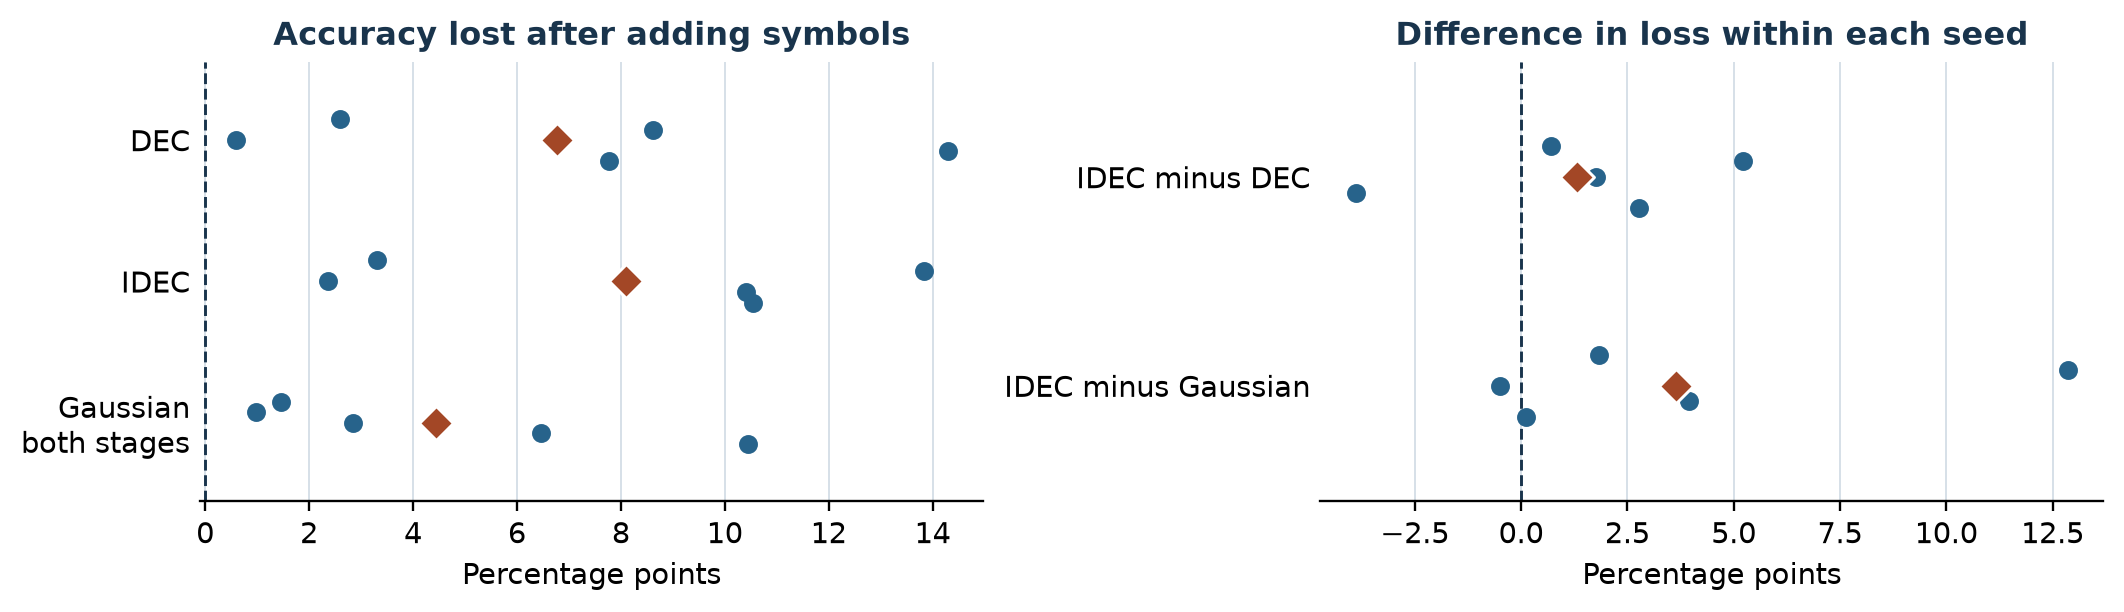
\includegraphics[width=.98\linewidth,height=.58\textheight,keepaspectratio]{../figures/dec_background_drops.png}
\par\medskip\normalsizeWith background symbols, DEC lost 6.77 accuracy points and IDEC lost 8.09. IDEC lost more in four of five seeds. The paired difference was $1.32\pm3.35$ points.

\notefoot{Dots are individual seeds. Diamonds are means. Positive values in the right panel mean ordinary IDEC lost more accuracy.}
\end{frame}

\begin{frame}{How do Gaussian weighting and translation compare?}
\centering\small\setlength{\tabcolsep}{4pt}\begin{tabular}{lrrrr}
\toprule
Method & Clean ACC & Marked ACC & Drop (pp) & Redraw flips\\
\midrule
DEC & 77.63 & 70.86 & 6.77 $\pm$ 5.40 & 3.19\\
IDEC & 73.23 & 65.14 & 8.09 $\pm$ 5.01 & 2.99\\
DEC + translation & 81.36 & 77.18 & 4.17 $\pm$ 4.04 & 2.34\\
IDEC + translation & 83.88 & 77.61 & 6.27 $\pm$ 2.74 & 1.78\\
Gaussian, both stages & 70.03 & 65.59 & 4.44 $\pm$ 3.98 & 2.63\\
Gaussian, pretraining only & 74.07 & 68.80 & 5.27 $\pm$ 4.64 & 2.62\\
Gaussian, fine-tuning only & 69.27 & 62.88 & 6.39 $\pm$ 5.18 & 3.20\\
KL only, random start & 31.00 & 28.90 & 2.10 $\pm$ 1.75 & 11.42\\
\bottomrule
\end{tabular}

\par\medskip\normalsizeTranslation raised IDEC accuracy by 12.47 points on marked digits and 10.65 on clean digits. Gaussian pretraining gave the highest marked accuracy among the weighted losses. Two-stage weighting narrowed the drop partly by lowering clean accuracy.

\notefoot{Translation moves the digit and both symbols together during pretraining. The drop is clean minus marked ACC, with the paired seed SD. Flips measure changes after a background redraw.}
\end{frame}

\begin{frame}{What the experiment tells us about relevance}
\key{Reconstruction contributes to the difficulty}\par
On identical marked inputs, the clean target improved accuracy in every seed. DEC also lost accuracy with symbols present. A 5.20-point gap was already visible at the shared autoencoder initialization.
\par\bigskip
\key{A Gaussian reduces the cost of peripheral errors}\par
With weighting in both stages, the decoder tracked the changed background less in every seed. Weighting only pretraining gave the best tradeoff among Gaussian variants here. The amount of background information retained in the code remains open.

\notefoot{A location prior assigns a large weight to a central distractor and a small weight to an off-center stroke. Transfer depends on how the objects of interest are positioned.}
\end{frame}
